\chapter{Hardware design}
The hardware chapter describes the different physical objects that have been designed and realized. 
\section{Power line and switch mode}
\writer{Dennis Madsen}
%
EPRO\_3\_\&\_4\_PLC - Hardware.pdf
\\ EEMC1 report
\p 

\section{Power switch}
\writer{Paulo Fontes}
%

\section{Interface}
\writer{Dennis Madsen}
According to chapter \ref{chap:digital_design} section \ref{sec:arm_to_fpga}, an interface board has been designed to connect the ARM processor with the FPGA. 
The design is described in \textit{time box 1}. Figure \ref{fig:arm2fpga_interface} shows the final mounted PCB
\p Beside interfacing the processor to the FPGA, the board also interfaces to the power line module. 
\p All unused pins from the pin headers J1 and J2 are routed to another pin header where some of the pins are used to control the power switches connected.
 
\begin{figure}[H]
	\begin{centering}
		 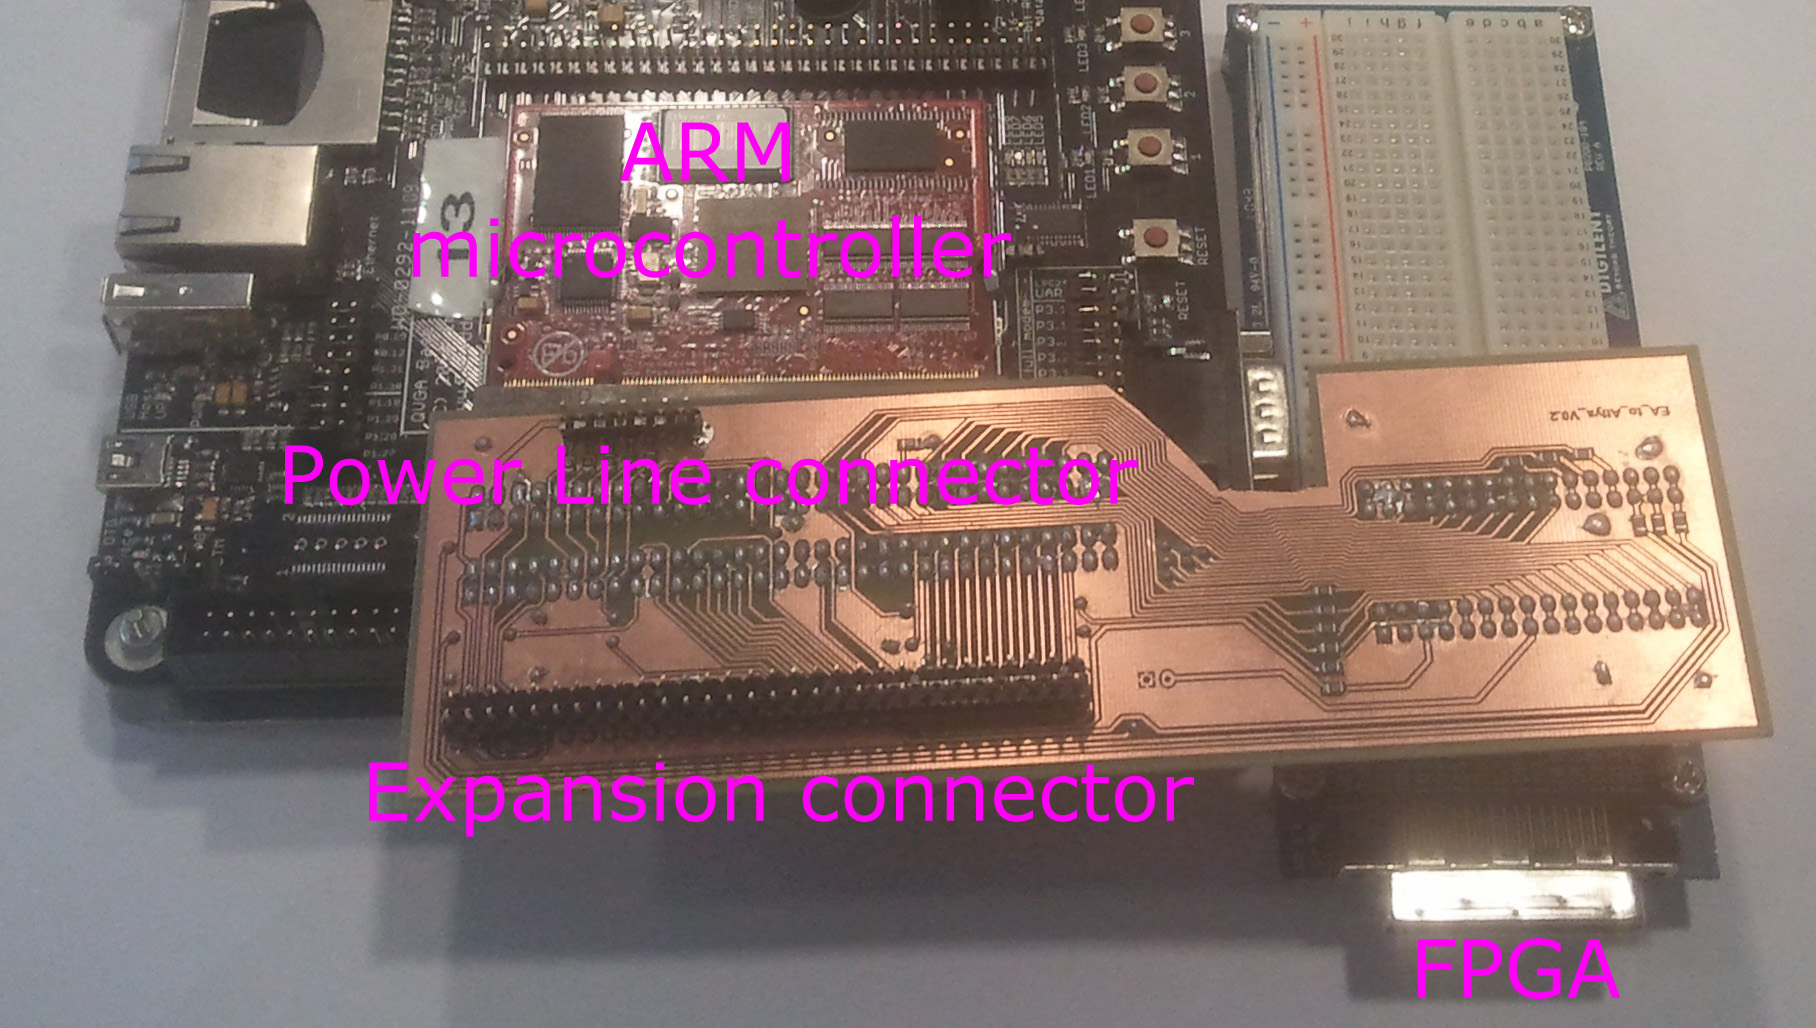
\includegraphics[width=0.80\textwidth]{images/hw_interface_photo_v0_2.jpg}
		\caption{Schematic of the ARM to Spartan6 connector, v0.2.}
		\label{fig:arm2fpga_interface}
	\end{centering}
\end{figure}
